\documentclass{article}

% Language setting
\usepackage[english, french]{babel}
\usepackage[T1]{fontenc} 
\usepackage[autolanguage]{numprint}

% Set page size and margins
\usepackage[a4paper,top=2cm,bottom=2cm,left=3cm,right=3cm,marginparwidth=1.75cm]{geometry}

% item
\usepackage{enumitem}

% Useful packages
\usepackage{amsmath,amssymb}
\usepackage{graphicx}
\usepackage[export]{adjustbox}
\usepackage[colorlinks=true, allcolors=blue]{hyperref}
\usepackage{multicol}
\usepackage{listings}
\usepackage{minted}

%\title{La Manipulation du Marché de l'Art}
%\title{Rapport DSB}
%\author{Florian EPAIN et Thomas De Premorel}
%\date{March 23, 2022}



\begin{document}

\begin{titlepage}
   \begin{center}
       \vspace*{1cm}
       \Huge
       \textbf{La Manipulation du Marché de l'Art}

       \vspace{0.5cm}
       \LARGE
        Rapport DSB
        
        \text{Groupe 2}
            
       \vspace{1.5cm}

       \textbf{Florian EPAIN}
       
       \text{florian.epain@etudiant.univ-rennes1.fr}
       
       \textbf{Thomas De Premorel}
       
       \text{???@etudiant.univ-rennes1.fr}
       
       \vspace{0.5cm}
       \text{March 23, 2022}

   \end{center}
   
   \vspace{13cm}
    \begin{abstract}
        C'est surement indigeste mais j'y ai mis mon coeur.
    \end{abstract}
\end{titlepage}



\tableofcontents
\clearpage

%%%%%%%%%%%%%%%%%%%%%%%%%%%%%%%%%%%%%%%%%%%%%%%%%%%%%%%%%%%%%%%%%%%%%%%%%%%%%%%%%%%%%%%%%%%%%%%%%%%%%%%%%%%%

\section{Introduction}

Nous avons choisi de représenter la 'discrimination' des artistes dans le marché de l'art et le principe d'évaluation d'une oeuvre d'art.

Depuis l'aube des temps, les artistes ont eu du mal à se rémunérer et ce phénomène est d'autant plus fort dans ce monde d'hyper-concurence et néocapitaliste.

D'après les dits de cette video : 
\begin{figure}[htp]
    \centering
    \href{https://www.youtube.com/watch?v=ZZ3F3zWiEmc}
    {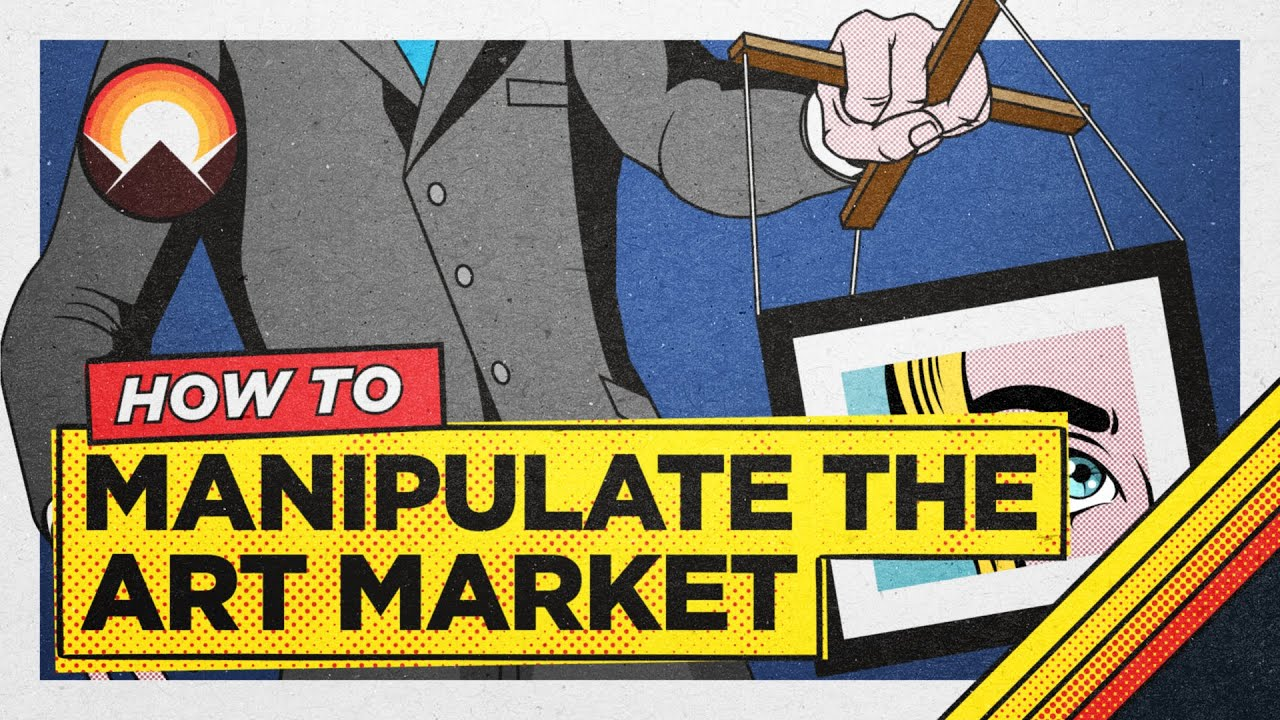
\includegraphics[width=0.5\textwidth]{miniature.jpeg}}
    \caption{\label{fig:miniature}The Art Market is a Scam (And Rich People Run It)}
\end{figure}

L'art n'a pas de valeur intrisèque.
L'art se voit etre évalué par la somme \emph{hypothétique} que les acheteurs \emph{potentiels} sont prêt à dépenser pour l'acquérir. Il en va donc d'une enchère monétaire, de manipulation de critique, mais aussi de recherche et de travaux d'expert sur certaines oeuvres pour que celle-ci se voit identifiée, voire authentifiée, ce qui a pour cause de monter son prix.
\\

Ce marché est très restreint, accessible uniquement par des strates très riches de nos sociétés. En effet, le prix d'entrée des marchés où se déroulent les ventes les plus 'lucratives' et onéreuses dépasse souvent le salaire moyen d'une vie d'un salarié (source dans un prochain épisode).

La grande majorité des ventes mondiales d'art sont concentrées à New york, Hong-kong et London.
\\

Le problème se pose sur le caractère spéculatif (stéril et fictif), subjectif et concentré de ce système. Ce sont dans ce genre de petit monde où le monopole contrôle tout (les prix, quand pour les ventes, combien d'oeuvre, etc) -> \href{https://youtu.be/ZZ3F3zWiEmc?t=895}{l'exemple} des oeuvres d'Andy Warhol et du presque unique acheteur Jose Mugrabi.

Ces mêmes conditions qu'a permit à Mugrabi de dominer le marché des oeuvres de Warhol, à son influence de fonctionner reflètent que la connivence et la corruption s'y confonde facilement.
\\

Nous parlons même pour le marché de l'art d'une composition d'arnaques, par exemple : \newline
Contre-intuitivement, d'ultra-riche individus peuvent gagner en rentabilité en procédant à des donations d'art.

    Pour le cas des US -se trouve également en France-, lorsqu'un de ces individus opère une donation d'art à un musée -à but non-lucratif- il obtient une déduction de taxe.
    
        Pour un don d'une oeuvre valant 10 millions de \$\, la déduction d'impôt s'applique pour 10 millions, qui en théorie devrait leur profiter de 4 millions.
    Etant donné la difficulté de determiner la valeur d'oeuvre, l'IRS (\href{https://www.irs.gov/}{Internal Revenue Service} : organisme de taxation des Etats Unis vis-à-vis de l'art) se voit surpayer 38\%\ des déductions de taxes comparement à la valeur établie plus tard. (source manquante dans la vidéo)
    
        En résumé, un ultra-riche pourrait acheter un pièce d'art pour 4millions.
        L'apprécier pendant quelque année, négocier pour une évaluation favorable, augmenter sa valeur, se baser sur le fait que l'IRS n'audite (ne contrôle) qu'une infime partie des oeuvres, faire la donation pour 10millions et il aura déjà atteint le seuil de rentabilité.
        
        Ce don aura également pour cause, la présence d'une piece d'une même collection dans le musée, d'augmenter le prix des autres de la collection que ce créancier possède potiellement (puissance d'un monopole).

\paragraph{L'art n'est plus un exercice de compétence, c'est celui d'une marque.}

%%%%%%%%%%%%%%%%%%%%%%%%%%%%%%%%%%%%%%%%%%%%%%%%%%%%%%%%%%%%%%%%%%%%%%%%%%%%%%%%%%%%%%%%%%%%%%%%%%%%%%%%%%%%

\section{Modèle conceptuel}


Nous avons omis les conservateurs de musée, propriétaire de gallerie et d'autres acteurs dans l'équation de l'évaluation du prix d'une oeuvre. 
Les relations de connaisance entre les différents humains, leur contact, leur société écran, \emph{etc.} 
Ce procédé reste complexe et non exhaustivement représenté par cette base de donnée.
Il s'agit surtout d'une ébauche.

\subsection{Description du modèle}

L'art est au milieu de tout ce système. 
Ce marché se compose de plusieurs acteurs, chacun influence la valeur de l'oeuvre.
Comme représenté sur ce shéma mocodo : \ref{fig:MCD_last}

Une pièce d'oeuvre d'art possède:
\begin{itemize}[label=\(\blacktriangleright\)]
    \item un numéro d'objet (unique);
    \item un titre;
    \item un medium (type);
    \item une cote (la valeur estimée de l'oeuvre).
\end{itemize}
Nous avons décidé de séparer le créateur de la pièce, étant donné que son créateur peut etre inconnu ou en avoir plusieurs.


\begin{multicols}{2}[]
Nombreuses tables représentent des humains, pour pouvoir les différencier nous les avons séparé en plusieurs tables.
Ces humains possèdent tous ces \emph{attributs fixes}:
\begin{itemize}[label=\(\blacktriangleright\)]
    \item un identifiant unique*;
    \item un nom;
    \item une nationalité.
\end{itemize}

Certains d'entre eux peuvent avoir comme attribut :
\begin{itemize}[label=\(\blacktriangleright\)]
    \item un capital;
    \item une spécialité;
    \item un site web;
    \item une réputation.
\end{itemize}
\end{multicols}


Les attributs des artistes sont tous facultatifs sauf leur identifiant qui lui est unique.
En effet, on va créer un profil artiste lorsqu'on retrouve une collection d'oeuvre à l'artiste inconnu, on les regroupe par un artiste 'fantôme'.
Ils possèdent potentiellement un site-web -un contact- et une réputation.
Cette réputation est positive, un artiste avec une réputation :
\begin{itemize}[label=\(\blacktriangleright\)]
    \item = 0 est inconnu;
    \item > 1000 est connu localement;
    \item > 2000 est connu à l'internationale;
    \item > 10000 est une figure historique.
\end{itemize}

On associe les artistes avec les artworks par la relation CREE.
Un Artwork peut etre créé par personne ou plusieurs artistes. Et un artiste peut ne rien avoir créé ou avoir une multitude de création.


Les Mecenes sont peu majoritaire dans le marche de l'art,
il s'agit surtout de créancier qui achetent directement à l'artiste. 
Ils possèdent les attributs humains fixes, une réputation (même ordre que celle des les artistes) et leur patrimoine supposé (capital).
Ces Mecènes peuvent ou pas AIDE un ou des artistes, représenté par une somme d'argent : montantAide 

    
\begin{multicols}{2}[]
Les Créanciers sont principalement des commerciaux plutôt que des collectionneurs d'art. 
Ils ont les attributs fixes et un capital.
Ils peuvent vendre de l'art, à un certain prix (prixVente), à un certain moment (dateDeVente).
Ils peuvent participer à un seul marché à la fois, dans lequel ils peuvent acheter/vendre des oeuvres répertoriée dans la relation PARTICIPE
Pour les achats de crénacier à créancier privé (sans marché public) on passe par vend et possede.
\\

    Les Commissaires-priseurs ont seulement les attributs fixes.
Ils peuvent diriger un marché. 

    Pour qu'une oeuvre monte en valeur, et s'affiche mieux dans un immense salon, les Restaurateurs travaillent avec les Musées, les galeries et les collectionneurs d'art (créancier).
Ils sont en contact direct avec les oeuvres (relation RESTAURE: pour un certain prix (prixRestauration)).
\\

    Les Critiques sont des personnes publiques émettant un jugement sur certaine oeuvre, mouvement d'art.
Ils jouent un rôle important dans la monter de prix des oeuvres (relation JUGE: en donnant une cote -coteDonnee-).
\end{multicols}

\clearpage

Enfin les Experts sont des chercheurs, en Histoire, en Matière, en Technique.
Leur collaboration avec le corps des galeries et créanciers est essentielle pour l'authentification d'oeuvre d'art.
Prouver qu'une pièce est l'original peut faire grimper sa cote de plusieurs millions. \cite{Christ's_Portrait}
\\

Le marché devra être dirigé par un commissaire-priseur et peut avoir aucun ou plusieurs créanciers participant.
Il s'agit de galerie privée, où le prix d'entrée (prixEntryMarche) vise à resteindre les acheteurs (n'avoir que la même 'clientèle').
Ils sont unique et ne durent que le jour dateMarche*.
Ces marchés peuvent être heberger par des organismes privés ou avoir des locaux fixes comme \href{https://fr.wikipedia.org/wiki/Christie's}{Christies's} ou \href{https://fr.wikipedia.org/wiki/Sotheby's}{Sotheby's}.
Il se déroule à un certain moment (dateMarche), rendez vous à ne pas manquer pour repérer les fluctuations de prix et certaines oeuvres qui peuvent se rentabiliser.
\\

Les Galeries et les Musées sont des organismes présentant des oeuvres (EXPOSE et PRET resp),
elles ne peuvent pas ouvrir si ces organismes n'ont pas assez d'oeuvres à exposer.

\href{https://fr.wikipedia.org/wiki/Musée}{D'après l'ICOM}, un musée est une institution permanente sans but lucratif au service de la société et de son développement ouverte au public, qui acquiert, conserve, étudie, expose et transmet le patrimoine matériel et immatériel de l’humanité et de son environnement à des fins d'études, d'éducation et de délectation. 
Le musée doit avoir une dateCreation* et une adresseMusee*.

Une galerie à une date de creation ou date d'evenement pour les galeries temporaires (dateGalerie).
Un prixEntryExpo, pouvant dépassant les centaines de milliers de dollars.
Une galerie peut reverser les gains à une association. (smiley qui sourit)
Une galerie peut être à l'extérieur, à l'intérieur dans des locaux fixes ou mobiles.



%\begin{figure}[htp]
%\centering 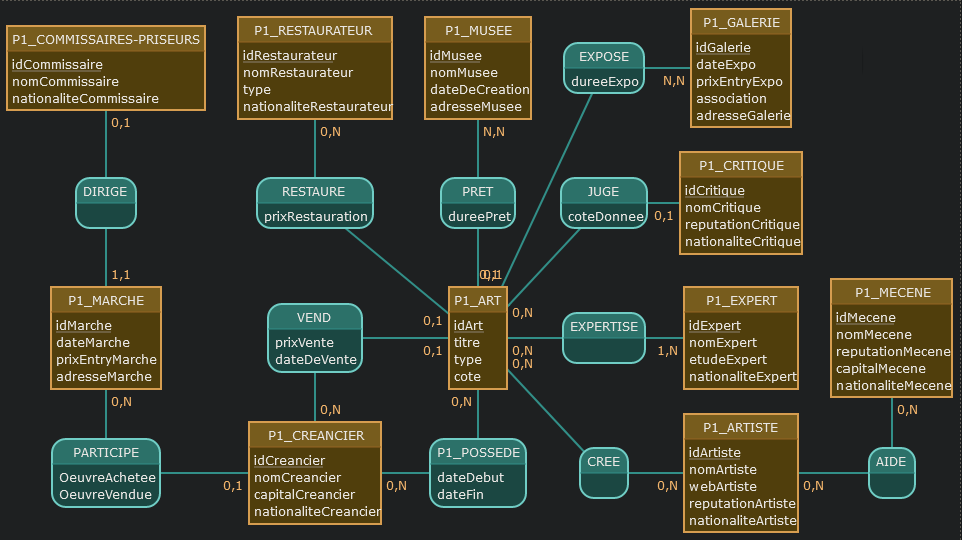
\includegraphics[width=1\textwidth]{mocodo_old.png} \caption{\label{fig:MCD_old}Ancien Schéma Mocodo.}
%\end{figure}

\begin{figure}[htp]
\centering
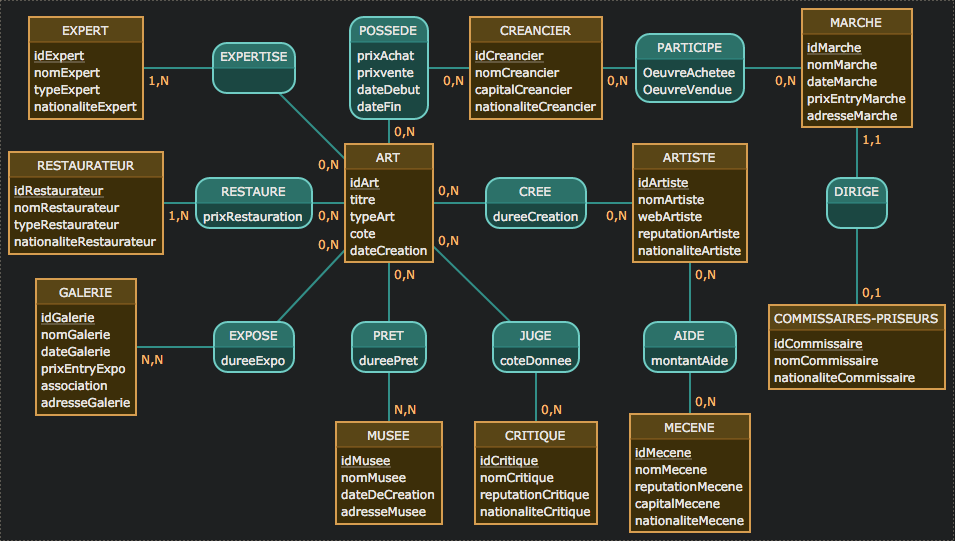
\includegraphics[width=1\textwidth]{new_mocodo.png}
\caption{\label{fig:MCD_last}Schéma Mocodo Revisité.}
\end{figure}


\clearpage

%%%%%%%%%%%%%%%%%%%%%%%%%%%%%%%%%%%%%%%%%%%%%%%%%%%%%%%%%%%%%%%%%%%%%%%%%%%%%%%%%%%%%%%%%%%%%%%%%%%%%%%%%%%%

\section{Modèle relationnel}
\subsection{Application règle 1}

ART ( \underline{idArt}, titre, typeArt, cote, dateCreation ) \newline
%pb : l'importation de la BDD MoMA met 0 à la place du vide pour bcp d'attrib
COMMISSAIRE-PRISEUR ( \underline{idCommissaire}, nomCommissaire*, nationaliteCommissaire )\newline
RESTAURATEUR ( \underline{idRestaurateur}, nomRestaurateur*, typeRestaurateur*, nationaliteRestaurateur )\newline
MUSEE ( \underline{idMusee}, nomMusee*, dateDeCreation*, adresseMusee )\newline
GALERIE ( \underline{idGalerie}, nomGalerie*, dateGalerie*, prixEntryExpo, association, adresseGalerie* )\newline
CRITIQUE ( \underline{idCritique}, nomCritique*, reputationCritique, nationaliteCritique )\newline
MARCHE ( \underline{idMarche}, nomMarche*, dateMarche*, prixEntryMarche, adresseMarche*)\newline
EXPERT ( \underline{idExpert}, nomExpert*, typeExpert*, nationaliteExpert )\newline
MECENE ( \underline{idMecene}, nomMecene*, reputationMecene, capitalMecene, nationaliteMecene )\newline
CREANCIER ( \underline{idCreancier}, nomCreancier*, capitalCreancier, nationaliteCreancier )\newline
ARTISTE ( \underline{idArtiste}, nomArtiste, webArtiste, reputationArtiste, nationaliteArtiste )\newline

\subsection{Application règle 2 et 2bis}

Les 0 1 et 1 1 se transforment en clé étrangères et supprime la relation qui est alors inutile.
Ici le marché étant unique, il n'est dirigé que par un seul commissaire-priseur, la relation dirige est alors incorporée dans la table marché.

MARCHE ( \underline{idMarche}, nomMarche*, dateMarche*, prixEntryMarche, adresseMarche*, \underline{\underline{idcommissaire}})

\subsection{Application règle 3}

Ces relations deviennent des tables contenant des clés étrangères pour permettre à toutes informations de pouvoir être accèder sans ambiguité.
Et les relations inutiles sont supprimées 
\\
PARTCIPE(\underline{\underline{idMarche}}*, \underline{\underline{idCreancier}}*, OeuvreAchetee, OeuvreVendue) \newline

OeuvreAch, et OeuvreVend correspondent à des idArt \newline
\\
POSSEDE(\underline{\underline{idCreancier}}*, \underline{\underline{idArt}}*, prixAchat, prixVente, dateDebut*, dateFin) \newline

Les deux relation POSSEDE et VEND sont fusionné afin d'éviter les conflits \newline
Le prix peut etre privé (sans trop d'interet dans le milieu de la spéculation) \newline
\\
RESTAURE(\underline{\underline{idRestaurateur}}*, \underline{\underline{idArt}}*, prixRestauration) \newline
PRET(\underline{\underline{idMusee}}*, \underline{\underline{idArt}}*, dureePret*) \newline
EXPOSE(\underline{\underline{idGalerie}}*, \underline{\underline{idArt}}*, dureeExpo*) \newline
JUGE(\underline{\underline{idCritique}}*, \underline{\underline{idArt}}*, coteDonnee*) \newline
EXPERTISE(\underline{\underline{idExpert}}*, \underline{\underline{idArt}}*) \newline
CREE(\underline{\underline{idArtiste}}*, \underline{\underline{idArt}}*, dureeCreation) \newline
AIDE(\underline{\underline{idMecene}}*, \underline{\underline{idArtiste}}*, montantAide) \newline


\clearpage

\newgeometry{left=0.5cm,right=0.5cm,top=0.5cm,bottom=1.5cm}
\section{Schéma physique}

\begin{multicols}{2}


\begin{minted}
{sql}
CREATE DATABASE IF NOT EXISTS `MERISE`
DEFAULT CHARACTER SET utf8
COLLATE utf8_general_ci;
USE `MERISE`;
DROP TABLE IF EXISTS POSSEDE;
DROP TABLE IF EXISTS CREE;
DROP TABLE IF EXISTS PARTICIPE;
DROP TABLE IF EXISTS EXPOSE;
DROP TABLE IF EXISTS RESTAURE;
DROP TABLE IF EXISTS PRET;
DROP TABLE IF EXISTS JUGE;
DROP TABLE IF EXISTS EXPERTISE;
DROP TABLE IF EXISTS AIDE;
DROP TABLE IF EXISTS CRITIQUE;
DROP TABLE IF EXISTS EXPERT;
DROP TABLE IF EXISTS ARTISTE;
DROP TABLE IF EXISTS MECENE;
DROP TABLE IF EXISTS RESTAURATEUR;
DROP TABLE IF EXISTS MUSEE;
DROP TABLE IF EXISTS GALERIE;
DROP TABLE IF EXISTS ART;
DROP TABLE IF EXISTS CREANCIER;
DROP TABLE IF EXISTS MARCHE;
DROP TABLE IF EXISTS COMMISSAIRE_PRISEUR;

CREATE TABLE ART (
  idart INT NOT NULL,
  titre VARCHAR(1000),
  typeArt VARCHAR(1000),
  cote VARCHAR(1000),
  dateCreation VARCHAR(1000),
  PRIMARY KEY (idart)
);

CREATE TABLE ARTISTE (
  idartiste INT NOT NULL,
  nomartiste VARCHAR(1000),
  webartiste VARCHAR(1000),
  reputationartiste INT,
  nationaliteartiste VARCHAR(1000),
  PRIMARY KEY (idartiste)
);

CREATE TABLE COMMISSAIRE_PRISEUR (
  idcommissaire INT NOT NULL,
  nomcommissaire VARCHAR(1000) NOT NULL,
  nationalitecommissaire VARCHAR(1000),
  PRIMARY KEY (idcommissaire)
);

CREATE TABLE MARCHE (
  idmarche INT NOT NULL,
  nommarche VARCHAR(1000) NOT NULL,
  datemarche DATE NOT NULL,
  prixentrymarche VARCHAR(1000),
  adressemarche VARCHAR(1000) NOT NULL,
  idcommissaire INT NOT NULL,
  PRIMARY KEY (idmarche),
  FOREIGN KEY (idcommissaire)
  REFERENCES COMMISSAIRE_PRISEUR(idcommissaire)
);


CREATE TABLE RESTAURATEUR (
  idrestaurateur INT NOT NULL,
  nomrestaurateur VARCHAR(1000) NOT NULL,
  typerestaurateur VARCHAR(100) NOT NULL,
  nationaliterestaurateur VARCHAR(42),
  PRIMARY KEY (idrestaurateur)
);

CREATE TABLE MUSEE (
  idmusee INT NOT NULL,
  nommusee VARCHAR(1000) NOT NULL,
  datedecreation DATE NOT NULL,
  adressemusee VARCHAR(1000) NOT NULL,
  PRIMARY KEY (idmusee)
);

CREATE TABLE GALERIE (
  idgalerie INT NOT NULL,
  nomgalerie VARCHAR(1000) NOT NULL,
  dategalerie DATE NOT NULL,
  prixentryexpo INT,
  association VARCHAR(1000),
  adressegalerie VARCHAR(1000) NOT NULL,
  PRIMARY KEY (idgalerie)
);

CREATE TABLE CRITIQUE (
  idcritique INT NOT NULL,
  nomcritique VARCHAR(1000) NOT NULL,
  reputationcritique INT,
  nationalitecritique VARCHAR(1000),
  PRIMARY KEY (idcritique)
);

CREATE TABLE EXPERT (
  idexpert INT NOT NULL,
  nomexpert VARCHAR(1000) NOT NULL,
  typeexpert VARCHAR(1000) NOT NULL,
  nationaliteexpert VARCHAR(1000),
  PRIMARY KEY (idexpert)
);

CREATE TABLE MECENE (
  idmecene INT NOT NULL,
  nommecene VARCHAR(1000) NOT NULL,
  reputationmecene INT,
  capitalmecene INT,
  nationalitemecene VARCHAR(1000),
  PRIMARY KEY (idmecene)
);

CREATE TABLE CREANCIER (
  idcreancier INT NOT NULL,
  nomcreancier VARCHAR(1000) NOT NULL,
  capitalcreancier INT,
  nationalitecreancier VARCHAR(1000),
  PRIMARY KEY (idcreancier)
);





CREATE TABLE POSSEDE (
  idcreancier INT NOT NULL,
  idart INT NOT NULL,
  prixAchat INT,
  prixVente INT,
  datedebut DATE NOT NULL,
  datefin DATE,
  PRIMARY KEY (idcreancier, idart),
  FOREIGN KEY (idart)
  REFERENCES ART(idart),
  FOREIGN KEY (idcreancier)
  REFERENCES CREANCIER(idcreancier)
);

CREATE TABLE CREE (
  idartiste INT NOT NULL,
  idart INT NOT NULL,
  PRIMARY KEY (idartiste, idart),
  FOREIGN KEY (idart)
  REFERENCES ART(idart),
  FOREIGN KEY (idartiste)
  REFERENCES ARTISTE(idartiste)
);

CREATE TABLE PARTICIPE (
  idcreancier INT NOT NULL,
  idmarche INT NOT NULL,
  oeuvreachetee INT,
  oeuvrevendue INT,
  PRIMARY KEY (idcreancier, idmarche),
  FOREIGN KEY (idcreancier)
  REFERENCES CREANCIER(idcreancier),
  FOREIGN KEY (idcreancier)
  REFERENCES MARCHE(idmarche),
    FOREIGN KEY (oeuvreachetee)
  REFERENCES ART(idart),
    FOREIGN KEY (oeuvrevendue)
  REFERENCES ART(idart)
);

CREATE TABLE EXPOSE (
  idart INT NOT NULL,
  idgalerie INT NOT NULL,
  dureeexpo DATE NOT NULL,
  PRIMARY KEY (idart, idgalerie),
  FOREIGN KEY (idart)
  REFERENCES ART(idart),
  FOREIGN KEY (idgalerie)
  REFERENCES GALERIE(idgalerie)
);


CREATE TABLE RESTAURE (
  idrestaurateur INT NOT NULL,
  idart INT NOT NULL,
  prixrestauration INT,
  PRIMARY KEY (idrestaurateur, idart),
  FOREIGN KEY (idart)
  REFERENCES ART(idart),
  FOREIGN KEY (idrestaurateur)
  REFERENCES RESTAURATEUR(idrestaurateur)
);

CREATE TABLE PRET (
  idart INT NOT NULL,
  idmusee INT NOT NULL,
  dureepret DATE NOT NULL,
  PRIMARY KEY (idart, idmusee),
  FOREIGN KEY (idart)
  REFERENCES ART(idart),
  FOREIGN KEY (idmusee)
  REFERENCES MUSEE(idmusee)
);

CREATE TABLE JUGE (
  idcritique INT NOT NULL,
  idart INT NOT NULL,
  cotedonnee INT NOT NULL,
  PRIMARY KEY (idcritique, idart),
  FOREIGN KEY (idart)
  REFERENCES ART(idart),
  FOREIGN KEY (idcritique)
  REFERENCES CRITIQUE(idcritique)
);

CREATE TABLE EXPERTISE (
  idexpert INT NOT NULL,
  idart INT NOT NULL,
  PRIMARY KEY (idexpert, idart),
  FOREIGN KEY (idart)
  REFERENCES ART(idart),
  FOREIGN KEY (idexpert)
  REFERENCES EXPERT(idexpert)
);

CREATE TABLE AIDE (
  idmecene INT NOT NULL,
  idartiste INT NOT NULL,
  PRIMARY KEY (idmecene, idartiste),
  FOREIGN KEY (idartiste)
  REFERENCES ARTISTE(idartiste),
  FOREIGN KEY (idmecene)
  REFERENCES MECENE(idmecene)
);
\end{minted}
\end{multicols}

\restoregeometry

\section{Peuplement des tables uwu}

\href{https://github.com/MuseumofModernArt/collection}{Github: Museum of Modern Art}

Nous avons utilisé seulement quelque informations contenues dans la base de données MoMA :
\\Pour les artistes :
\begin{itemize}[label=\(\blacktriangleright\)]
    \item DisplayName (leur nom);
    \item Nationality (leur origine).
\end{itemize}
Pour les oeuvres d'art :
\begin{itemize}[label=\(\blacktriangleright\)]
    \item Title;
    \item Artist;
    \item Medium;
    \item Date de création.
\end{itemize}

Toutes les autres informations contenues dans notre base de données
n'est que pure supposition et imagination (cote d'une oeuvre / reputation d un artiste / \emph{etc})


\subsection{Artistes}

On importe
\hyperref[]{}{}

\subsection{Artworks}
\subsection{Humains Qquonque}
\subsection{Relations}


\section{Requetes SQL}

\subsection{Projection}

\LaTeX{} is great at typesetting mathematics. Let $X_1, X_2, \ldots, X_n$ be a sequence of independent and identically distributed random variables with $\text{E}[X_i] = \mu$ and $\text{Var}[X_i] = \sigma^2 < \infty$, and let
\[S_n = \frac{X_1 + X_2 + \cdots + X_n}{n}
      = \frac{1}{n}\sum_{i}^{n} X_i\]
denote their mean. Then as $n$ approaches infinity, the random variables $\sqrt{n}(S_n - \mu)$ converge in distribution to a normal $\mathcal{N}(0, \sigma^2)$.


\subsection{Jointure}

Usually the template you're using will have the page margins and paper size set correctly for that use-case. For example, if you're using a journal article template provided by the journal publisher, that template will be formatted according to their requirements. In these cases, it's best not to alter the margins directly.

If however you're using a more general template, such as this one, and would like to alter the margins, a common way to do so is via the geometry package. You can find the geometry package loaded in the preamble at the top of this example file, and if you'd like to learn more about how to adjust the settings, please visit this help article on \href{https://www.overleaf.com/learn/latex/page_size_and_margins}{page size and margins}.

\subsection{Moyenne sur l'integralite d'un attribut}

Overleaf supports many different languages, including multiple different languages within one document. 

To configure the document language, simply edit the option provided to the babel package in the preamble at the top of this example project. To learn more about the different options, please visit this help article on \href{https://www.overleaf.com/learn/latex/International_language_support}{international language support}.

To change the spell check language, simply open the Overleaf menu at the top left of the editor window, scroll down to the spell check setting, and adjust accordingly.

\subsection{Regroupement par calcul}

You can simply upload a \verb|.bib| file containing your BibTeX entries, created with a tool such as JabRef. You can then cite entries from it, like this: \cite{greenwade93}. Just remember to specify a bibliography style, as well as the filename of the \verb|.bib|. You can find a \href{https://www.overleaf.com/help/97-how-to-include-a-bibliography-using-bibtex}{video tutorial here} to learn more about BibTeX.

If you have an \href{https://www.overleaf.com/user/subscription/plans}{upgraded account}, you can also import your Mendeley or Zotero library directly as a \verb|.bib| file, via the upload menu in the file-tree.

\subsection{Différence}

We hope you find Overleaf useful, and do take a look at our \href{https://www.overleaf.com/learn}{help library} for more tutorials and user guides! Please also let us know if you have any feedback using the Contact Us link at the bottom of the Overleaf menu --- or use the contact form at \url{https://www.overleaf.com/contact}.

\subsection{Division}

\subsection{Group By}

\section{Code}

\subsection{convert\_artists()}
\begin{minted}
{rust}

#[derive(Serialize, Deserialize, Debug)]
struct Artist {
	constituent_id: i128,
	display_name: String,
	artist_bio: Option<String>,
	nationality: Option<String>,
	gender: Option<String>,
	begin_date: i16,
	end_date: i16,
	wiki_qid: Option<String>, 
	ulan: Option<String>
}

fn convert_artists() -> Result<()>
{
    let path = "E:/Code/projects Rust/MoMA/Artists-reformed.json";

    let content = fs::read_to_string(path)
        .expect("Unable to read file");

    println!("-----read_.json-----");
	
    let artists: Vec<Artist> = serde_json::from_str(&content).unwrap();

    println!("--------create_request---------");

    let mut foo =
    "INSERT INTO P1_ARTISTE (idartiste, nomartiste, webartiste, reputationartiste, nationaliteartiste)
    \n VALUES ".to_string();

    for artist in artists
    {
        let artist_nationality: &str=
		match &artist.nationality {
			Some(s) => s,
			None => "",
		};

        //
        let mut artist_web = artist.display_name
            .replace(" ", ".").replace("'", "").replace(",","");
        artist_web.push_str(".org");

        let foobar =
        "\n (id,'display_name','site', reputation,'nationality')";
        let mut artist_n = foobar.replace("id", &artist.constituent_id.to_string());
        artist_n = artist_n.replace("display_name", &artist.display_name.replace("'", " "));
        artist_n = artist_n.replace("site", &artist_web);
        artist_n = artist_n.replace("reputation", &create_fictional_human::create_reputation(0,0).to_string());
        artist_n = artist_n.replace("nationality", &artist_nationality.replace("'", " "));
        foo.push_str(&artist_n);
        
        foo.push(','); // have to remove the last one
    }
    
    foo.push_str(";END"); //to end the SQL request
    foo = foo.replace(",;END",";");

    println!("--------create_.sql---------");

    // "/private/student/n/in/fepain/R/art-manipulation/RENDU/insert_artists.txt"
    // "E:/Code/projects Rust/art-manipulation/RENDU/insert_artists.txt"
	fs::write("E:/Code/projects Rust/art-manipulation/RENDU/insert_artists.sql",
			 foo)
		.expect("Unable to write file");

    Ok(())
}

\end{minted}

\bibliographystyle{alpha}
\bibliography{sample}

\end{document}